\documentclass[handout]{beamer}
\usepackage[utf8]{inputenc}
\usepackage[T1]{fontenc}
\usepackage[french]{babel} 
\usepackage{color}
\usepackage{fancyhdr}
\usepackage{lmodern} 
\usepackage{makeidx}
\usepackage{graphicx}
\usepackage{amsmath}
\usepackage{amssymb}
\usepackage{mathrsfs}
\usepackage[bottom]{footmisc}
\usepackage{float}
\usepackage{listings}
\usepackage{textcomp}
\usepackage{verbatim}
\usepackage{ulem}

\lstset{literate={é}{{\'e}}1}

\expandafter\def\expandafter\insertshorttitle\expandafter{%
	\insertshorttitle\hfill%
	\insertframenumber\,/\,\inserttotalframenumber}



\setbeamertemplate{blocks}[rounded]
\setbeamertemplate{footline}[frame number]
\usetheme{Warsaw}
\usefonttheme{serif}

\setbeamertemplate{headline}
{%
	\leavevmode%
	\begin{beamercolorbox}[wd=.5\paperwidth,ht=2.5ex,dp=1.125ex]{section in head/foot}%
		\hbox to .5\paperwidth{\hfil\insertsectionhead\hfil}
	\end{beamercolorbox}%
	\begin{beamercolorbox}[wd=.5\paperwidth,ht=2.5ex,dp=1.125ex]{subsection in head/foot}%
		\hbox to .5\paperwidth{\hfil\insertsubsectionhead\hfil}
	\end{beamercolorbox}%
}

\usecolortheme{whale}
\useoutertheme{split}

\title{Formation \LaTeX}
\author{KI '020}
\institute{Ecole des Ponts Paristech}
\date{\today}

\newif\ifplacelogo % condition pour le logo
\placelogotrue 
\logo{\ifplacelogo
\includegraphics[height=10mm]{Images/Logo_020}\fi}

\begin{document}
	
	
	\begin{frame}
		\titlepage
	\end{frame}
	
	\begin{frame}
		\frametitle{Sommaire}
		\setcounter{tocdepth}{1}
		\tableofcontents
	\end{frame}
	
	

	
	
	
	\section{Introduction}
	
		\begin{frame}
			\frametitle{Qu'est-ce que \LaTeX ?}
			
			\begin{tabular}{cc}
				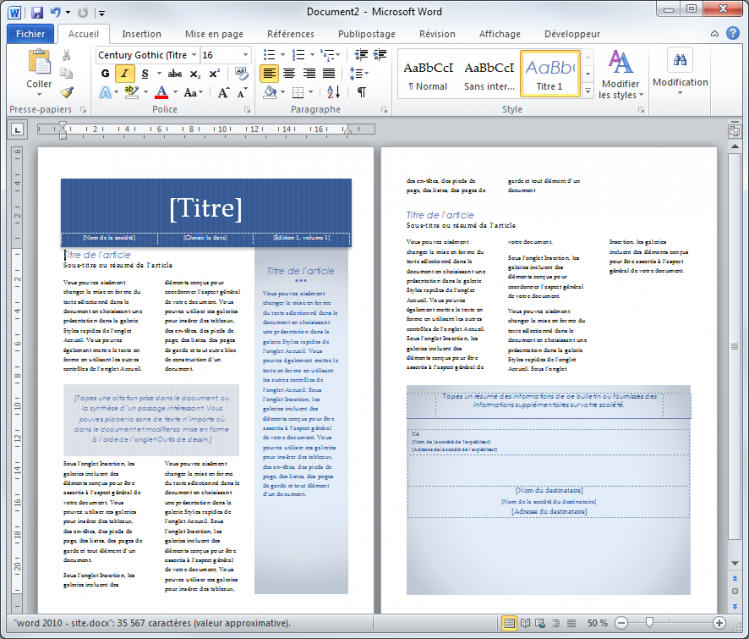
\includegraphics[width=5cm]{Images/Introduction/Word}&\includegraphics[width=5cm]{Images/Introduction/Latex}\\
				Word & \LaTeX
			\end{tabular}
	
		\end{frame}
	
		\begin{frame}
			\frametitle{Comment ça marche ?}
			
			\begin{tabular}{ccc}
				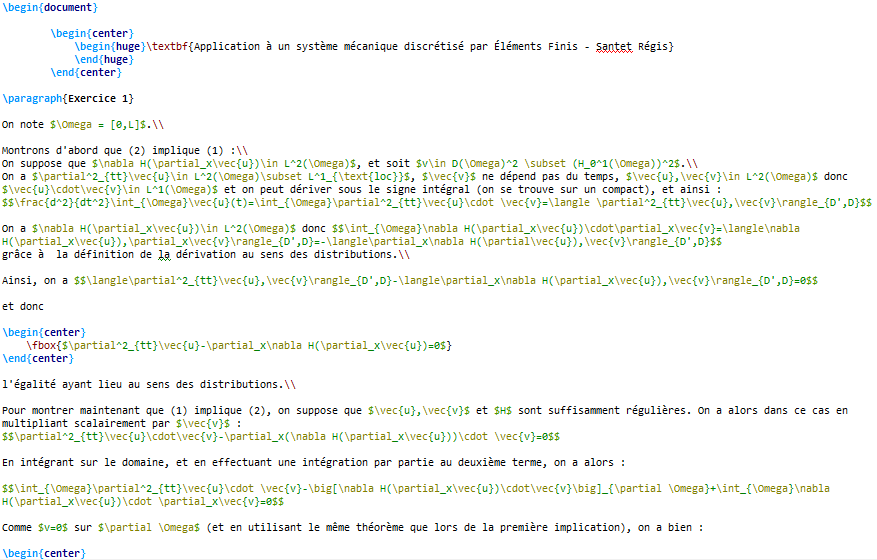
\includegraphics[width=5cm]{Images/Introduction/fichier_tex} & &
				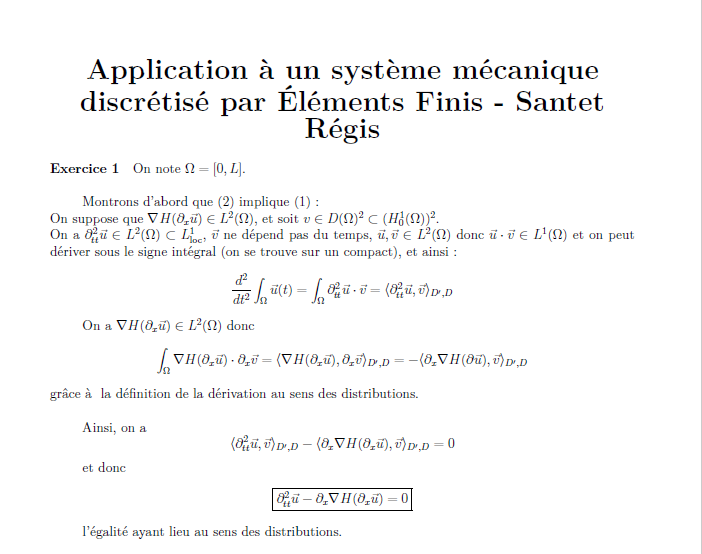
\includegraphics[width=5cm]{Images/Introduction/fichier_PDF}\\
				Fichier .tex & $\longrightarrow$ & Fichier PDF
			\end{tabular}
			
		\end{frame}
	
		\begin{frame}
			\frametitle{ShareLaTeX}
			
			\centering
			\textbf{SHARELATEX}\\
			HTTPS://FR.SHARELATEX.COM/
			
			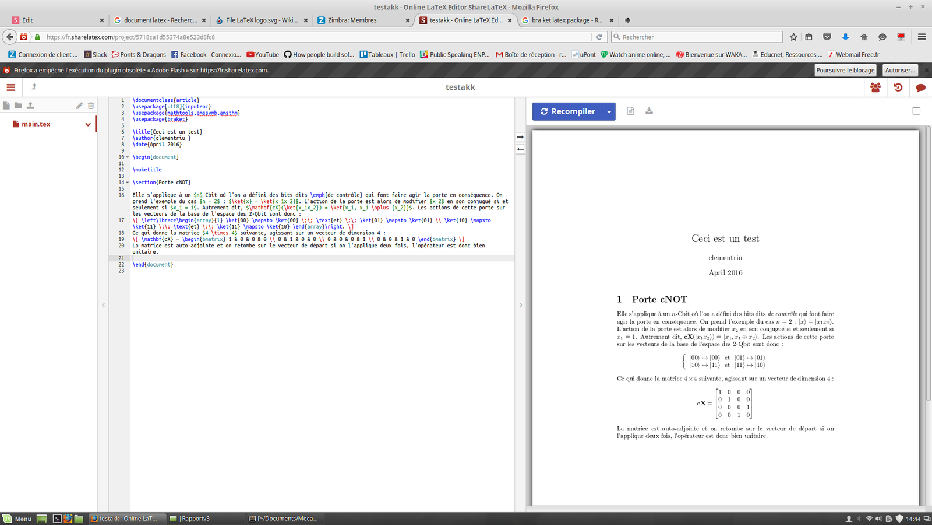
\includegraphics[width=0.8\linewidth]{Images/Introduction/sharelatex}
			
		\end{frame}
	
	
	
	
	\section{Créer un document \LaTeX}
	
	
		
		\begin{frame}[fragile=singleslide]
			\frametitle{LA commande}
			
			\begin{center}
				\huge
				Au commencement, il y avait la commande
			\end{center}
			
			\Huge
			\begin{block} 
				
			\begin{verbatim}
				\nom_commande{...}
			\end{verbatim}
			\end{block}
		\end{frame}
	
	\placelogofalse
	
		\begin{frame}[fragile=singleslide]
			\frametitle{La base d'un document \LaTeX}
			
			\begin{center}
				\Large
				Et la lumière fut...
			\end{center}
			\footnotesize
			\begin{block}
				
			\begin{verbatim}
			\documentclass[11pt,a4paper]{article}
			
			\usepackage[utf8]{inputenc}
			\usepackage[T1]{fontenc}
			\usepackage[french]{babel}
			\usepackage{lmodern}
			\usepackage{mathtools,amssymb}
			\usepackage{float}
			
			\title{Mon super titre}
			\author{Moi}
			\date{Aujourd'hui}
			
			\begin{document}
			
			\end{document}
			\end{verbatim}
			\end{block}
		\end{frame}
	
	\placelogotrue
	
		\begin{frame}[fragile=singleslide]
			\frametitle{Ca, c'est la classe}
			
			\Large
			\begin{block}
				
			\begin{verbatim}
			\documentclass[11pt,a4paper]{article}
			\end{verbatim}
			\end{block}
		\end{frame}
	
		\begin{frame}[fragile=singleslide]
			\frametitle{Beaucoup de packages}
			
			\LARGE
			\begin{block} 
				
			\begin{verbatim}
			\usepackage[utf8]{inputenc}
			\usepackage[T1]{fontenc}
			\usepackage[french]{babel}
			\usepackage{lmodern}
			\usepackage{mathtools,amssymb}
			\usepackage{float}
			\end{verbatim}
			\end{block}
		\end{frame}

		\begin{frame}[fragile=singleslide]
			\frametitle{Coucou c'est moi avec mon document}
			
			\huge
			\begin{block} 
				
			\begin{verbatim}
			\title{Mon super titre}
			\author{Moi}
			\date{Aujourd'hui}
			\end{verbatim}
			\end{block}
		\end{frame}
	
		\begin{frame}[fragile=singleslide]
			\frametitle{Ce qui encadre le tout}
			
			\huge
			\begin{block} 
				
			\begin{verbatim}
			\begin{document}
			
			\end{document}
			\end{verbatim}
			\end{block}
			
		\end{frame}

	
	\section{Mettre en forme le texte}
	
		\begin{frame}[fragile=singleslide]
			\frametitle{Structurons}
			\begin{block} 
				
			\begin{verbatim}
				\maketitle
				
				\part{Ma Partie}
				
				\section{Ma Section}
				\section*{Ma Section}
				
				\subsection{Sous-section}
				\subsubsection{Sous-sous-section}
				
				\paragraph{Mon paragraphe}
			\end{verbatim}
			\end{block}
		\end{frame}
	
		\begin{frame}
			
			\begin{center}
			
\includegraphics[scale=0.6]{Images/Structure/maketitle}
			\end{center}
			
		\end{frame}
	
		\begin{frame}
		
				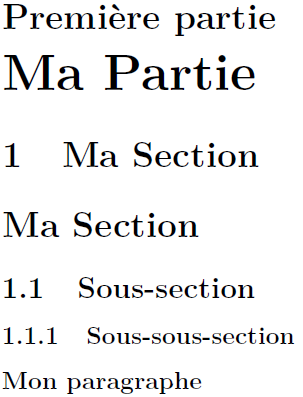
\includegraphics[width=4cm]{Images/Structure/structure}
				
		\end{frame}
	
		\begin{frame}[fragile=singleslide]
			\frametitle{Je veux tout sauter}
			
			\begin{center}
				Les commandes de tous les instants
			\end{center}
			
			\begin{block} 
				
			\begin{verbatim}
			\newline
			
			\\
			
			\indent 
			
			\newpage
			\end{verbatim}
			\end{block}
		\end{frame}
	
		\begin{frame}[fragile=singleslide]
			\frametitle{Listons}
			
\begin{minipage}[c]{6cm}
	\begin{block} 
		
	\begin{lstlisting}
\begin{itemize}
\item Bonjour
\item J'aime
\item Les
\item Pizzas
\end{itemize}
	
\begin{enumerate}
\item JE 
\item VEUX
\item DES
\item PIZZAS
\end{enumerate}
	\end{lstlisting} 
	\end{block}
\end{minipage} \hfill
\begin{minipage}[c][0cm]{4cm}
	\begin{center}
		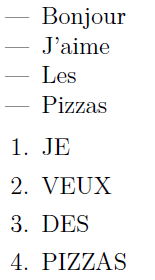
\includegraphics[width=2cm]{Images/Structure/item}
	\end{center}
\end{minipage}
			
		\end{frame}
	
	
		\begin{frame}[fragile=singleslide]
			\frametitle{Écrivons}
			
\begin{minipage}[c]{5cm}
	\begin{block} 
		
\begin{lstlisting}


\textbf{gras}

\textit{italique}

\texttt{script}

\underline{souligne}

\emph{emphase}

\textsc{Small Caps}

\fbox{encadre}
\end{lstlisting} 
\end{block}
\end{minipage} \hfill
\begin{minipage}[c][0cm]{5cm}
	\begin{center}
		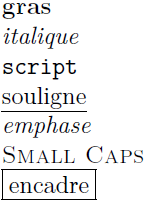
\includegraphics[width=2.5cm]{Images/Structure/ecrivons}
	\end{center}
\end{minipage}			


		\end{frame}
	
		\begin{frame}[fragile=singleslide]
			\frametitle{Commandes supplémentaires}
			
\begin{minipage}[c]{6cm}
\footnotesize
\begin{block} 
	
\begin{lstlisting}
\begin{quote}	
Citation
\end{quote}

\begin{quotation}
Citation
sur plusieurs lignes
\end{quotation}

Creer une note \footnote
{Voici une note de bas de page}

\end{lstlisting}
\end{block}
\end{minipage}\hfill
\begin{minipage}[c][0cm]{4cm}
	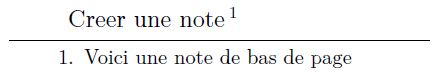
\includegraphics[width=4cm]{Images/Structure/footnote}
\end{minipage}

			
			
		\end{frame}
	
		\begin{frame}[fragile=singleslide]
			\frametitle{Commandes supplémentaires}
\scriptsize
\begin{block} 
	
\begin{lstlisting}
\begin{flushleft}  \begin{center}	  \begin{flushright}
Gauche		   Centre		  Droite
\end{flushleft}	   \end{center}	   	  \end{flushright}
\end{lstlisting}			
\end{block}
			
			
		\end{frame}
	
		\begin{frame}
			\frametitle{TP1}
			\centering
			
\includegraphics[width=10cm,height=8cm]{Images/Structure/TP1}
		\end{frame}

\placelogofalse
	
		\begin{frame}[fragile=singleslide]
			\frametitle{Solution}
		\footnotesize
		\begin{block} 
			
		\begin{verbatim}
		documentclass[11pt,a4paper]{article}
		
		\usepackage[utf8]{inputenc}
		\usepackage[T1]{fontenc}
		\usepackage[french]{babel}
		\usepackage{lmodern}
		\usepackage{mathtools,amssymb}
		\usepackage{float}
		
		\title{Pourquoi j'aime la formation \LaTeX}
		\author{KI '020}
		\date{\today}
		
		\begin{document}
		
		\maketitle
		\end{verbatim}
		\end{block}
	
		\end{frame}
	
	
		\begin{frame}[fragile=singleslide]
			\frametitle{Solution}
			
		\begin{block} 
			
		\begin{verbatim}
		\section{Parce que je trouve LaTeX cool}
		
		\LaTeX est purement un \textit{plaisir} à utiliser. 
		C'est aussi facile que de faire du vélo. 
		Sauf que le vélo est en feu. 
		Et que la route est en feu. 
		Et que je suis en enfer.\\
		\indent Je peux par exemple :
		\begin{itemize}
		\item \underline{Souligner} des machins 
		(\textbf{Such power !})
		\item Créer des \textsc{FUCKING NOTES DE BAS DE PAGE}
		\footnote{Et oui.} !
		\end{itemize}
		\end{verbatim}
		\end{block}
		
		\end{frame}
	
		\begin{frame}[fragile=singleslide]
		\frametitle{Solution}
		\begin{block} 
			
		\begin{verbatim}
		\subsection{Parce que je trouve le présentateur 
		awesome}

J'ai envie de lui écrire des poèmes en allemand. 
C'est très perturbant.

\section*{Autres raisons moins importantes}

\begin{enumerate}
\item Parce qu'il y a des \underline{\textsc{pizzas}}
\item aw yisss pizzas
\item om nom nom nom
\end{enumerate}
		\end{verbatim}
		\end{block}
		
		\end{frame}
	
	
	\section{Compléments} % (Références, tableaux, insérer du code, bibliographie, sommaire,...)

\placelogotrue
	
		\begin{frame}[fragile=singleslide]
			\frametitle{On dit merci qui ?}
			\centering \LARGE
			Faire des références
			\begin{block} 
				
			\begin{verbatim}
			\label{petit_nom}
			
			\ref{petit_nom}
			\end{verbatim}
			\end{block}
		\end{frame}
	
		\begin{frame}[fragile=singleslide]
			\frametitle{On dit merci qui ?}
			\begin{block} 
				
			\begin{verbatim}
			\section{Ma premiere section}
			\label{premiere_section}
			
			\section{Ma deuxieme section}
			
			Je fais reference a la section \ref{premiere_section}.
			\end{verbatim}
			\end{block}
			\centering
			
			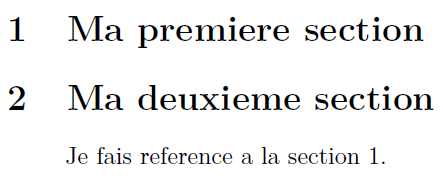
\includegraphics[width=5cm]{Images/Complements/reference}
			
		\end{frame}
	
	\placelogofalse
	
		\begin{frame}[fragile=singleslide]
			\frametitle{Ajout d'images}*
			\begin{block} 
				
			\begin{verbatim}
			...
			\usepackage{graphicx}
			\usepackage{float}
			...
			
			...
			\begin{figure}[H]
				\begin{center}
					\includegraphics[scale=...]{chemin}
					\caption{Description}
				\end{center}
			\end{figure}
			\end{verbatim}
			\end{block}
		\end{frame}
	
	\placelogotrue
	
		\begin{frame}[fragile=singleslide]
			\frametitle{Ajout de tableaux}
			\begin{block}
				
			\begin{verbatim}
\begin{tabular}{|c|c|c|}
\hline
a & b & c \\
\hline 
d & e & f \\
\hline 
bonjour & pizzas ? & pizzas \\
\hline
\end{tabular}
			\end{verbatim}
			\end{block}
			\centering
			
			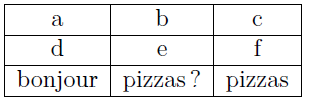
\includegraphics[width=5cm]{Images/Complements/tableau}
			
		\end{frame}
	
		\begin{frame}
			\frametitle{Ajout de tableaux}
			
			\centering
			
			\fbox{HTTP://WWW.TABLESGENERATOR.COM}
			
			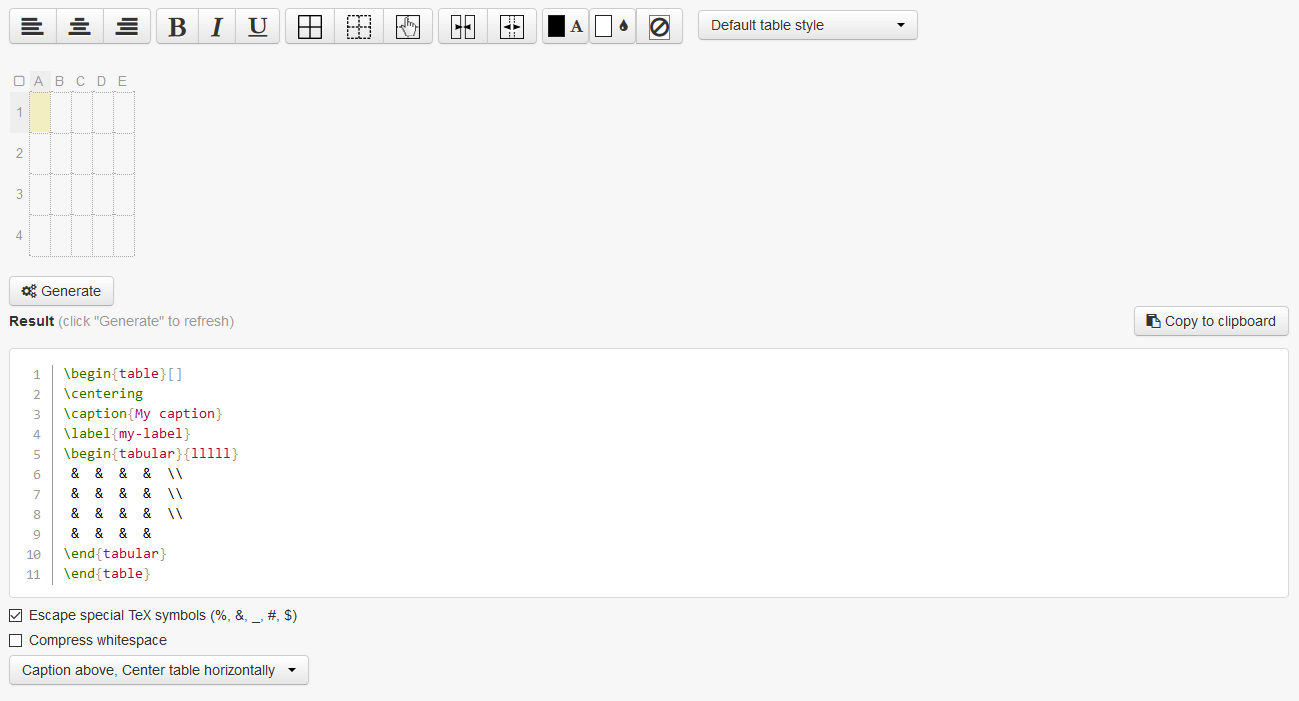
\includegraphics[width=10cm]{Images/Complements/tablesgenerator}
		\end{frame}
	
		\begin{frame}[fragile=singleslide]
			\frametitle{Insérer du code}
		\begin{block}	
			
			\begin{verbatim}
			...
			\usepackage{listings}
			...
			\lstset{language=Python,commentstyle=\color{gray},
			keywordstyle=\color{red},
			stringstyle=\color{blue},morekeywords={plt,np},
			breaklines=true}
			...
			\begin{lstlisting}
			code
			\end{lstlisting}
			\end{verbatim}
		\end{block}	
		\end{frame}
	
		\begin{frame}
			\frametitle{Insérer du code}
\centering
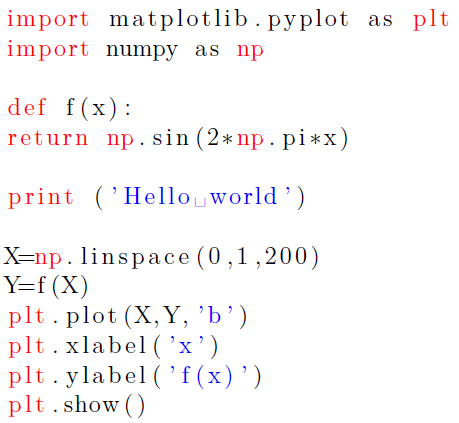
\includegraphics[width=7cm]{Images/Complements/code}
			
		\end{frame}
	
		\begin{frame}[fragile=singleslide]
			\frametitle{Sommaire}	
		
		\begin{center}
			Tout d'abord :
		\end{center}
	\begin{block}
			
		\begin{verbatim}
		\tableofcontents
		\end{verbatim}
	\end{block}	

		\begin{center}
			Pour changer "Table des matières" en "Mon nouveau titre" :
		\end{center}
	
	\begin{block}	
		
		\begin{verbatim}
		\renewcommand{\contentsname}{Mon nouveau titre} 
		\end{verbatim}
	\end{block}	

		\begin{center}
			Pour ne pas garder les sous--sous-sections :
		\end{center}
	
	\begin{block}
		
		\begin{verbatim}
		\setcounter{tocdepth}{2}
		\end{verbatim}
		
	\end{block}	
		\centering
		\begin{tabular}{|c|c|c|c|}
			\hline
			-1 & Partie & 3 & Sous-sous-section\\ \hline
			0 & Chapitre & 4 & Paragraphe \\ \hline
			1 & Section & 5 & Sous-paragraphe \\ \hline
			2 & Sous-section & & \\ \hline
		\end{tabular}
	
		\end{frame}
	
		\begin{frame}
			\frametitle{Ajout de la bibliographie}
			
		\end{frame}
	
		\begin{frame}
			\Huge
			\centering
			
			PAUSE <3 
		\end{frame}
	
	\section{Écrire des mathématiques}
	
	\begin{frame}[fragile=singleslide]
		\frametitle{Les packages}
		
		\centering
		Il nous faut :
		
		\begin{block}
			
			\begin{verbatim}
			...
			\usepackage{mathtools}
			\usepackage{amssymb}
			...
			\end{verbatim}
		\end{block}
		
		
		\centering
		\LaTeX contient déjà de nombreux outils pour les maths.\\
		Ces deux packages contiennent (presque) tout le reste.
	\end{frame}
	
	\begin{frame}[fragile=singleslide]
		\frametitle{L'environnement mathématique}
		
		
		\begin{block}
			
			\begin{verbatim}
			Soit $z$ un complexe. Alors $\cos^2(z)+\sin^2(z)=1$.
			\end{verbatim}
		\end{block}
	
	\vspace*{1cm}
	
	\centering 
	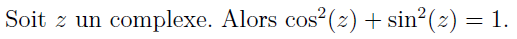
\includegraphics[width=8cm]{Images/Mathematiques/environnement1}
	
	\vspace*{1cm}
	
	L'environnement mathématique possède ses propres règles, ses propres commandes, sa propre police.
	
	\end{frame}

	\begin{frame}[fragile=singleslide]
		\frametitle{L'environnement mathématique}
		
		\begin{block}
			
			\begin{verbatim}
			Soit $z$ un complexe. Alors $$\cos^2(z)+\sin^2(z)=1$$
			\end{verbatim}
		\end{block}
		
		\vspace*{1cm}
		
		\centering 
		
\includegraphics[width=9cm]{Images/Mathematiques/environnement2}
		
	\end{frame}

	\begin{frame}[fragile=singleslide]
	\frametitle{L'environnement mathématique}
	
	\begin{block}
		
		\begin{verbatim}
		Soit $z$ un complexe. Alors 
		\begin{equation}
		\cos^2(z)+\sin^2(z)=1
		\end{equation}
		\end{verbatim}
	\end{block}
	
	\vspace*{1cm}
	
	\centering 
	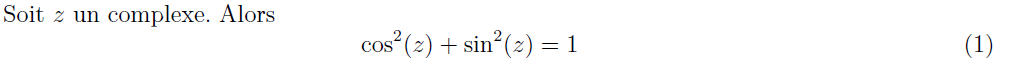
\includegraphics[width=9cm]{Images/Mathematiques/environnement3}
	
	\end{frame}
	
	\begin{frame}[fragile=singleslide]
		\frametitle{Écrivons les mathématiques}
		
	\begin{minipage}[c]{7cm}
		\begin{block} 
			
\begin{lstlisting}
\frac{num}{den}
base^{esposant}
base_{indice}
\sum_{bas}^{haut} terme
\prod_{bas}^{haut} facteur
\end{lstlisting} 

		\end{block}
	\end{minipage} \hfill
	\begin{minipage}[c][0cm]{3cm}
		\begin{center}
			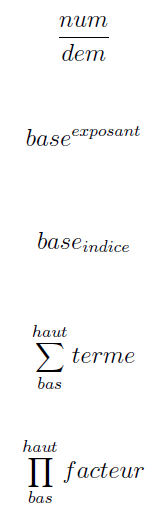
\includegraphics[width=2.3cm]{Images/Mathematiques/maths1}
		\end{center}
	\end{minipage}
		
	\end{frame}

	\begin{frame}[fragile=singleslide]
	\frametitle{Écrivons les mathématiques}
	
	\begin{minipage}[c]{7cm}
		\begin{block} 
			
\begin{lstlisting}
\sqrt{nombre}
\sqrt[n]{nombre}
\lim_{x \to a}
\int_{bas}^{haut} intégrande
\iint_{bas}^{haut} intégrande
\end{lstlisting} 
			
		\end{block}
	\end{minipage} \hfill
	\begin{minipage}[c][0cm]{3cm}
		\begin{center}
			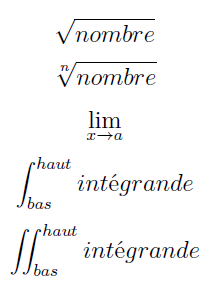
\includegraphics[width=3cm]{Images/Mathematiques/maths2}
		\end{center}
	\end{minipage}
	
	\end{frame}

	\begin{frame}[fragile=singleslide]
		\frametitle{Quelques symboles spéciaux}
		
\begin{minipage}[c]{7cm}
	\centering
	Les lettres grecques 
	
	\begin{block}
		
		\begin{verbatim}
		\alpha \beta \gamma
		\Omega \Lambda \Psi
		\end{verbatim}
	\end{block}
	
	\vspace*{1cm}
	
	Les glyphes mathématiques
	
	\begin{block}
		
		\begin{verbatim}
		\forall \exists \in
		\to \infty \partial
		\mathbb{R} \mathcal{N} \mathbf{I}
		\end{verbatim}
	\end{block}
\end{minipage}\hfill 
\begin{minipage}{3cm}
	\vspace*{1cm}
	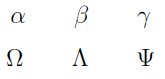
\includegraphics[width=2.5cm]{Images/Mathematiques/lettresgrecques}\vspace*{1.6cm}
	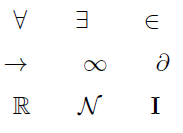
\includegraphics[width=2.5cm]{Images/Mathematiques/glyphes}
\end{minipage}

		
	\end{frame}

	\begin{frame}
		\frametitle{TP2}
	\begin{flushleft}
		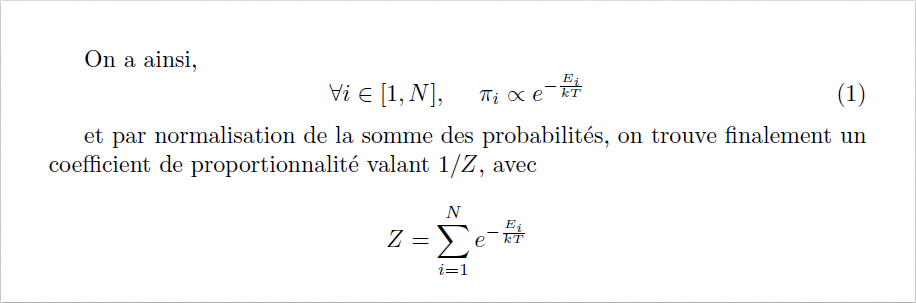
\includegraphics[width=11cm]{Images/Mathematiques/tp2}	
	\end{flushleft}
	

	\end{frame}

	\begin{frame}[fragile=singleslide]
		\frametitle{Solution}
		\begin{block}
			
			\begin{verbatim}
			On a ainsi,
			\begin{equation}
			\forall i \in [1,N], \ \ \ \ \pi_i 
			\propto e^{-\frac{E_i}{kT}}
			\end{equation}
			
			et par normalisation de la somme des probabilités, 
			on trouve finalement un 
			coefficient de proportionnalité valant $1/Z$, avec 
			$$ Z = \sum_{i=1}^{N}e^{-\frac{E_i}{kT}} $$
			\end{verbatim}
		\end{block}
	\end{frame}
	
	\begin{frame}[fragile=singleslide]
		\frametitle{Les matrices}
\begin{minipage}[c]{5cm}	
	\begin{block}
		
		\begin{verbatim}
		$$
		\begin{matrix}
		a & b & c\\
		d & e & f\\
		g & h & i
		\end{matrix}
		$$
		\end{verbatim}
	\end{block}
\end{minipage}\hfill
\begin{minipage}[c][0cm]{5cm}
	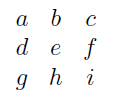
\includegraphics[width=2cm]{Images/Mathematiques/matrix1}
\end{minipage}
		
	\end{frame}
	
	\begin{frame}[fragile=singleslide]
		\frametitle{Les matrices}
\begin{minipage}[c]{5cm}	
	\begin{block}
		
		\begin{verbatim}
		$$
		\begin{pmatrix}
		a & b & c\\
		d & e & f\\
		g & h & i
		\end{pmatrix}
		$$
		\end{verbatim}
	\end{block}
\end{minipage}\hfill
\begin{minipage}[c][0cm]{5cm}
	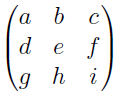
\includegraphics[width=2cm]{Images/Mathematiques/matrix2}
\end{minipage}
		
	\end{frame}
	
	\begin{frame}[fragile=singleslide]
		\frametitle{Les matrices}
\begin{minipage}[c]{5cm}	
	\begin{block}
		
		\begin{verbatim}
		$$
		\begin{bmatrix}
		a & b & c\\
		d & e & f\\
		g & h & i
		\end{bmatrix}
		$$
		\end{verbatim}
	\end{block}
\end{minipage}\hfill
\begin{minipage}[c][0cm]{5cm}
	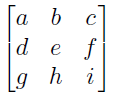
\includegraphics[width=2cm]{Images/Mathematiques/matrix3}
\end{minipage}
		
	\end{frame}

	\begin{frame}[fragile=singleslide]
	\frametitle{Les matrices}

\begin{minipage}[c]{5cm}	
	\begin{block}
		
		\begin{verbatim}
		$$
		\begin{vmatrix}
		a & b & c\\
		d & e & f\\
		g & h & i
		\end{vmatrix}
		$$
		\end{verbatim}
	\end{block}
\end{minipage}\hfill
\begin{minipage}[c][0cm]{5cm}
	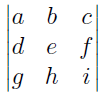
\includegraphics[width=2cm]{Images/Mathematiques/matrix4}
\end{minipage}
	
	\end{frame}

	\begin{frame}[fragile=singleslide]
		\frametitle{Remplir les matrices}	
		
		Mais on remplit avec quoi alors ?
		
		\begin{itemize}
			\item Des chiffres, des lettres, des symboles,...
			\item Beaucoup de points : 
			\begin{itemize}
				\item \begin{verbatim}
				\cdots
				\end{verbatim}, points horizontaux
				\item \begin{verbatim}
						\vdots
						\end{verbatim}, points verticaux
				\item \begin{verbatim}
				\ddots 
				\end{verbatim}, points diagonaux
			\end{itemize}
			\item Des espaces, pour des questions d'alignement : \begin{verbatim}
			a \phantom{bc} d
			\end{verbatim}
		
		\end{itemize}
	
	\centering
	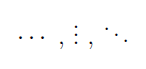
\includegraphics[width=3cm]{Images/Mathematiques/points}
		
	\end{frame}	

	\begin{frame}[fragile=singleslide]
		\frametitle{Les systèmes d'équations}

\begin{minipage}[c]{5cm}	
	\begin{block}
		
		\begin{verbatim}
			$$
\left\{
\begin{array}{ccc}
gauche1 &=& droite1\\
gauche2 &=& droite2\\
gauche3 &=& droite3
\end{array}
\right.
$$
		\end{verbatim}
	\end{block}
\end{minipage}\hfill
\begin{minipage}[c][0cm]{5cm}
	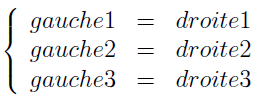
\includegraphics[width=3cm]{Images/Mathematiques/systeme}
\end{minipage}	
		
	\end{frame}

	\begin{frame}
		\frametitle{TP3}
		\begin{flushleft}
			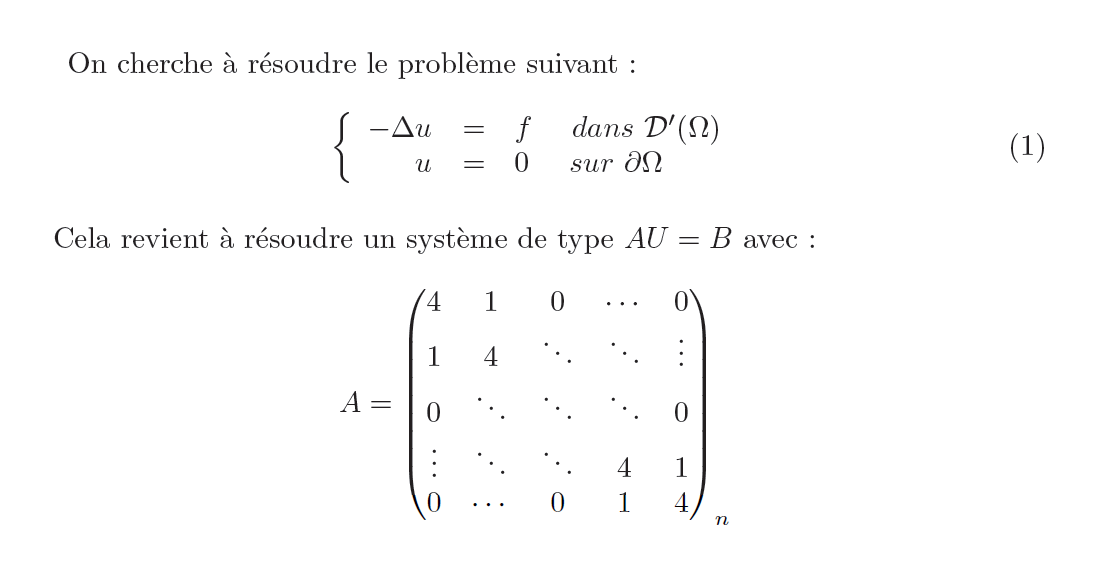
\includegraphics[width=10.5cm]{Images/Mathematiques/tp3}	
		\end{flushleft}
	\end{frame}

	\begin{frame}[fragile=singleslide]
		\frametitle{Solution}
		
		\begin{block}
			
			\begin{verbatim}
			On cherche à résoudre le problème suivant :
			\begin{equation}
			\left\{
			\begin{array}{r c l c}
			-\Delta & = & f & dans ~ \mathcal{D}'(\Omega)\\
			u & = & 0 & sur ~ \partial \Omega
			\end{array}
			\right.
			\end{equation}
			\end{verbatim}
		\end{block}
		
	\end{frame}

	\begin{frame}[fragile=singleslide]
		\frametitle{Solution}
		
		\begin{block}
			
			\begin{verbatim}
			\paragraph{}Cela revient à résoudre un système 
			de type $AU=B$ avec :
			$$
			A = 
			\begin{pmatrix}
			4      & 1      & 0      & \cdots & 0      \\
			1      & 4      & \ddots & \ddots & \vdots \\
			0      & \ddots & \ddots & \ddots & 0      \\
			\vdots & \ddots & \ddots & 4      & 1      \\
			0      & \cdots & 0      & 1      & 4
			\end{pmatrix}_n
			$$
			\end{verbatim}
		\end{block}
	\end{frame}

	
	\begin{frame}
		\centering
		\Huge
		"Google est votre ami !" 
	\end{frame}

\section{Ouverture}

	\begin{frame}
		\frametitle{Pour l'avenir}
		\framesubtitle{De nouveaux environnements}
		
		\centering
		\sout{\textsc{SHARELATEX}}
		
		\begin{itemize}
			\item IDE : Miktex, Texmaker, Kile (avec texlive)
		\end{itemize}
	\end{frame}

	\begin{frame}
	\frametitle{Pour l'avenir}
	\framesubtitle{Des compilateurs et éditeurs dédiés}
	
	\centering
	\sout{\textsc{SHARELATEX}}
	
	\begin{itemize}
		\item IDE : Miktex, Texmaker, Kile (avec texlive)
		\item Compilateur / éditeur : texlive / Vim, Emacs, Atom, Gedit, Notepad++
	\end{itemize}
	\end{frame}

	\begin{frame}
	\frametitle{Pour l'avenir}
	\framesubtitle{Des outils plus complexes}
	
	\centering
	\sout{\textsc{SHARELATEX}}
	
	\begin{itemize}
		\item IDE : Miktex, Texmaker, Kile (avec texlive)
		\item Compilateur / éditeur : texlive / Vim, Emacs, Atom, Gedit, Notepad++
		\item Les .sty et le CTAN (classes, extensions, packages)
	\end{itemize}
	\end{frame}

	\begin{frame}
	\frametitle{Pour l'avenir}
	\framesubtitle{Des outils plus complexes}
	
	\centering
	\sout{\textsc{SHARELATEX}}
	
	\begin{itemize}
		\item IDE : Miktex, Texmaker, Kile (avec texlive)
		\item Compilateur / éditeur : texlive / Vim, Emacs, Atom, Gedit, Notepad++
		\item Les .sty et le CTAN (classes, extensions, packages)
		\item Tex, LaTeX, BibTeX, LuaLaTeX, XeTeX (langages de scripts \textit{lua}, mise en page en \textit{Unicode})
	\end{itemize}
	\end{frame}

	\begin{frame}
		\frametitle{Un éditeur d'image ?}
		\framesubtitle{Tikz et pgf}
		
		\begin{minipage}{6cm}
			
			\begin{itemize}
				\item Des dessins, des graphes, ...\\
				\texttt{http://www.texample.net/media/
					tikz/examples/PDF/
					phasor-diagram.pdf}
			\end{itemize}
		\end{minipage}\hfill
		\begin{minipage}{4cm}
			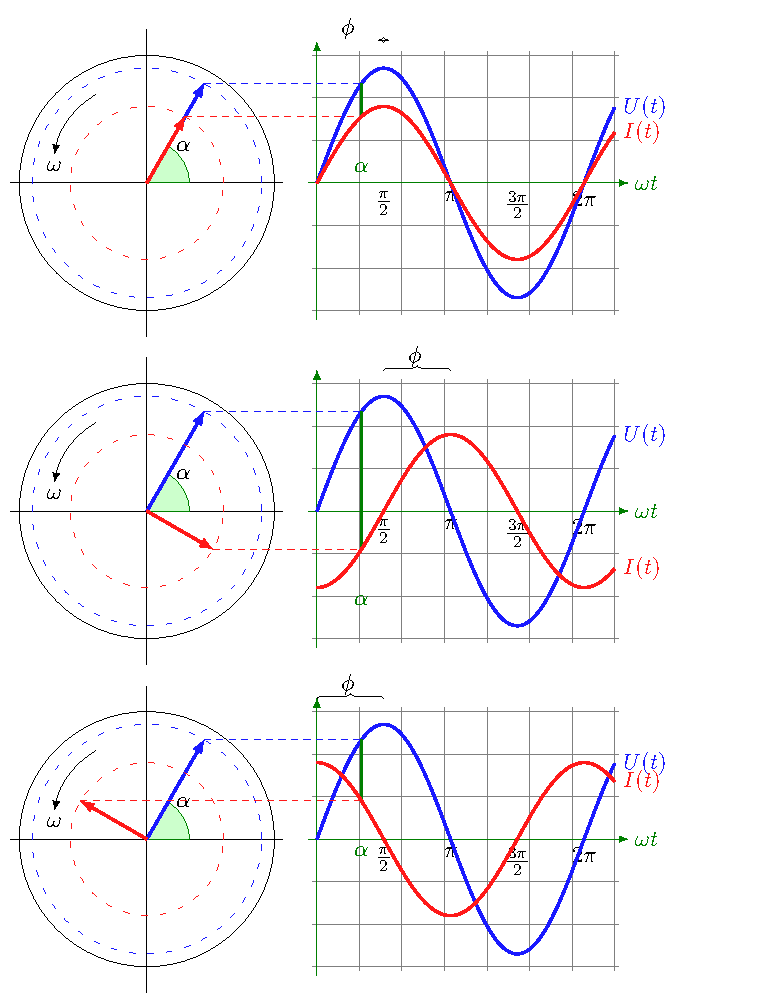
\includegraphics[width=4cm]{Images/Ouverture/phasor_diagram}
		\end{minipage}
	
		
	\end{frame}

	\begin{frame}
	\frametitle{Un éditeur d'image ?}
	\framesubtitle{Tikz et pgf}
	
	\begin{minipage}{6cm}
		
		\begin{itemize}
			\item Des dessins, des graphes, ...\\
			\texttt{http://www.texample.net/media/
				tikz/examples/PDF/
				phasor-diagram.pdf}
			\item Exportation géogébra
		\end{itemize}
	\end{minipage}\hfill
	\begin{minipage}{4cm}
		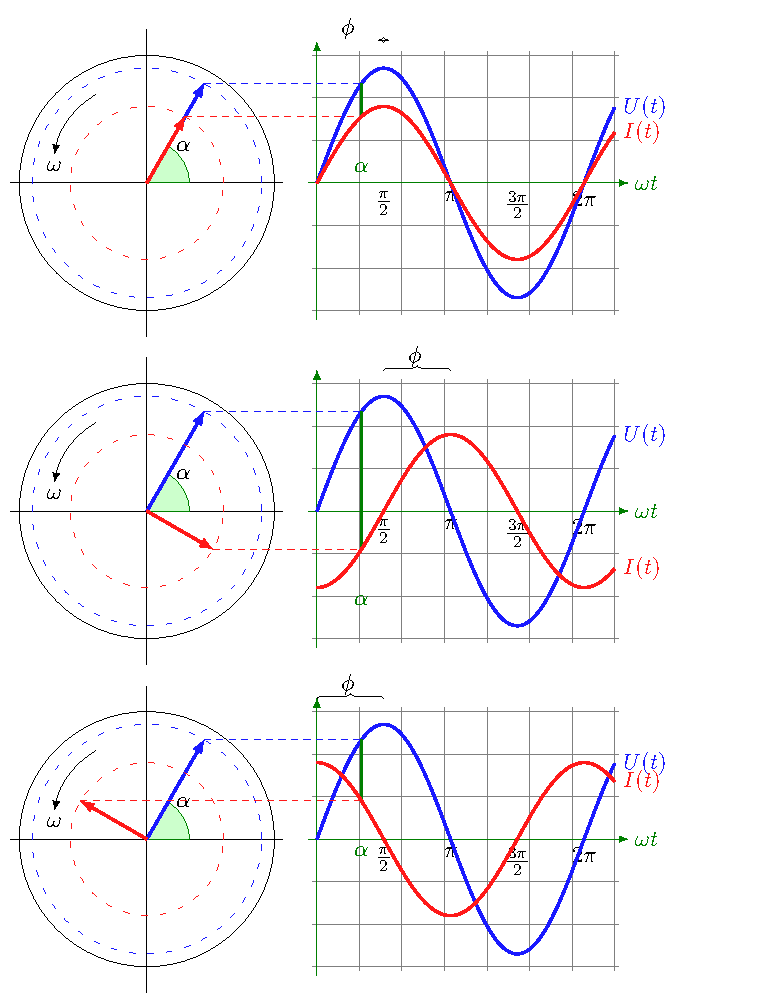
\includegraphics[width=4cm]{Images/Ouverture/phasor_diagram}
	\end{minipage}
	
	
	\end{frame}

	\begin{frame}[fragile=singleslide]
		\frametitle{Les présentations}
		\framesubtitle{Comment faire une présentation aussi stylée ?}
		
		\begin{itemize}
			\item Ces slides sont faites en \LaTeX avec le type \textbf{beamer}\\
			\begin{block}
				
				\begin{verbatim}
				\begin{frame}
				\frametitle{Titre de la slide}
				Contenu de la slide
				\end{frame}
				\end{verbatim}
			\end{block}
		\end{itemize}
	
	\end{frame}

	\begin{frame}[fragile=singleslide]
		\frametitle{Les présentations}
		\framesubtitle{Comment faire une présentation aussi stylée ?}
		
		\begin{itemize}
			\item Ces slides sont faites en \LaTeX avec le type \textbf{beamer}\\
			\begin{block}
				
				\begin{verbatim}
				\begin{frame}
				\frametitle{Titre de la slide}
				Contenu de la slide
				\end{frame}
				\end{verbatim}
			\end{block}
		
			\item L'environnement double colonne, minipage,...
			\begin{block}
				
				\begin{verbatim}
				\begin{columns}
				\begin{column}[c]{5cm} ... \end{column}
				\begin{column}[c]{4cm} ... \end{column}
				\end{columns}
				\end{verbatim}
			\end{block}
			
		\end{itemize}
		
	\end{frame}
	
	\begin{frame}[fragile=singleslide]
		\frametitle{Python avec \LaTeX}
	
\begin{minipage}{6cm}
	\begin{itemize}
		\item \LaTeX dans Matplotlib : r' '\\
		\begin{lstlisting}
plt.title(r'$\sin(2\pi x)$ 
sur $[0,1]$')
		\end{lstlisting}
	\end{itemize}
\end{minipage}\hfill
\begin{minipage}{4cm}
	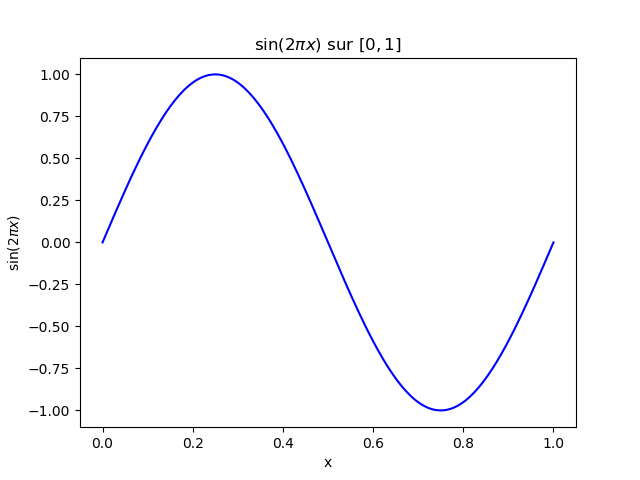
\includegraphics[width=4cm]{Images/Ouverture/python_latex}
\end{minipage}

	\end{frame}

	\begin{frame}[fragile=singleslide]
	\frametitle{Python avec \LaTeX}
	
	\begin{minipage}{6cm}
		\begin{itemize}
			\item \LaTeX dans Matplotlib : r' '\\
			\begin{lstlisting}
plt.title(r'$\sin(2\pi x)$ 
sur $[0,1]$')
			\end{lstlisting}
			\item Changer la police, la taille,...\\
			\texttt{https://matplotlib.org/users
				/usetex.html}
		\end{itemize}
	\end{minipage}\hfill
	\begin{minipage}{4cm}
		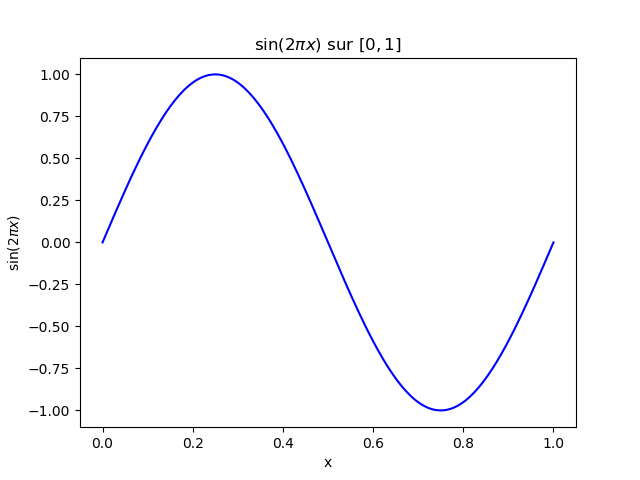
\includegraphics[width=4cm]{Images/Ouverture/python_latex}
	\end{minipage}

		
	\end{frame}
	
	\begin{frame}[fragile=singleslide]
		\frametitle{Python avec \LaTeX}
		
		\begin{minipage}{6cm}
			\begin{itemize}
				\item \LaTeX dans Matplotlib : r' '\\
				\begin{lstlisting}
plt.title(r'$\sin(2\pi x)$ 
sur $[0,1]$')
				\end{lstlisting}
				\item Changer la police, la taille,...\\
				\texttt{https://matplotlib.org/users
					/usetex.html}
				\item Exporter de belles figures\\
				\texttt{plt.savefig('output.eps',format='eps',dpi=1000)}
			\end{itemize}
		\end{minipage}\hfill
		\begin{minipage}{4cm}
			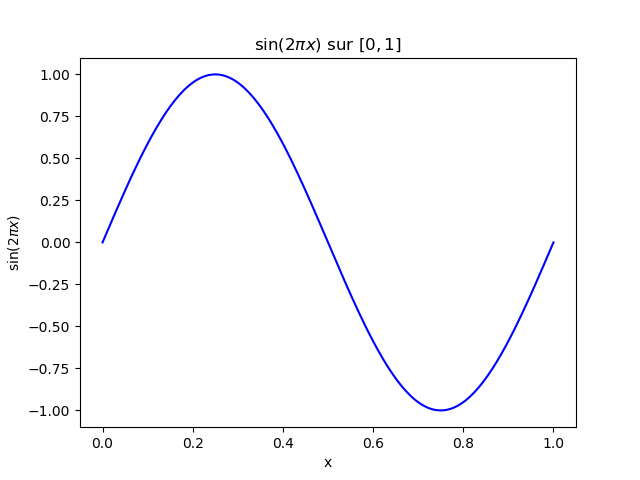
\includegraphics[width=4cm]{Images/Ouverture/python_latex}
		\end{minipage}
		
		
	\end{frame}

	\begin{frame}[fragile=singleslide]
		\frametitle{Jupyter Notebook}
		
		Exporter un notebook en latex depuis notebook avec du bash :
		\begin{block}
			
		\begin{verbatim}
		%%bash 
		jupyter nbconvert notebook.ipynb --to latex
		latex notebook.tex
		pdflatex notebook.tex
		\end{verbatim}
		\end{block}
	\end{frame}

	\begin{frame}[fragile=singleslide]
		\frametitle{Formatage des paragraphes}
		
		\begin{itemize}
			\item Changer les marges  de la page\\
			\begin{block}
			
			\begin{verbatim}
			\usepackage[a4paper,total={6in,8in}]{geometry}
			\end{verbatim}
			\end{block}
		\end{itemize}
	\end{frame}

	\begin{frame}[fragile=singleslide]
	\frametitle{Formatage des paragraphes}
	
	\begin{itemize}
		\item Changer les marges  de la page\\
		\begin{block}
			
		\begin{verbatim}
		\usepackage[a4paper,total={6in,8in}]{geometry}
		\end{verbatim}
		\end{block}
		\item Indentation d'un paragraphe\\
		\begin{block}
			
		\begin{verbatim}
		\setlength{\parindent}{4em}
		\end{verbatim}
		\end{block}
	\end{itemize}
	\end{frame}

	\begin{frame}[fragile=singleslide]
	\frametitle{Formatage des paragraphes}
	
	\begin{itemize}
		\item Changer les marges  de la page\\
		\begin{block}
			
		\begin{verbatim}
		\usepackage[a4paper,total={6in,8in}]{geometry}
		\end{verbatim}
		\end{block}
		\item Indentation d'un paragraphe\\
		\begin{block}
			
		\begin{verbatim}
		\setlength{\parindent}{4em}
		\end{verbatim}
		\end{block}
		\item Distance inter-paragraphe\\
		\begin{block}
			
		\begin{verbatim}
		\setlength{\parskip}{1em}
		\end{verbatim}
		\end{block}
	\end{itemize}
	\end{frame}

	\begin{frame}[fragile=singleslide]
	\frametitle{Formatage des paragraphes}
	
	\begin{itemize}
		\item Changer les marges  de la page\\
		\begin{block}
			
		\begin{verbatim}
		\usepackage[a4paper,total={6in,8in}]{geometry}
		\end{verbatim}
		\end{block}
		\item Indentation d'un paragraphe\\
		\begin{block}
			
		\begin{verbatim}
		\setlength{\parindent}{4em}
		\end{verbatim}
		\end{block}
		\item Distance inter-paragraphe\\
		\begin{block}
			
		\begin{verbatim}
		\setlength{\parskip}{1em}
		\end{verbatim}
		\end{block}
		\item Hauteur de ligne\\
		\begin{block}
			
		\begin{verbatim}
		\renewcommand{\baselinestretch}{2}
		\end{verbatim}
		\end{block}
	\end{itemize}
	\end{frame}

	\begin{frame}[fragile=singleslide]
		\frametitle{Mettre un lien}
		
		\begin{enumerate}
			\item Include le module :\\
			\begin{block}
				
			\begin{verbatim}
			\usepackage{hyperref}
			\end{verbatim}
			\end{block}
		\end{enumerate}
	\end{frame}

	\begin{frame}[fragile=singleslide]
	\frametitle{Mettre un lien}
	
	\begin{enumerate}
		\item Include le module :\\
		\begin{block}
			
		\begin{verbatim}
		\usepackage{hyperref}
		\end{verbatim}
		\end{block}
		\item Faire des liens :\\
		\begin{block}
			
		\begin{verbatim}
		\url{https://en.wikibooks.org/wiki/LaTeX}
		\href{https://en.wikibooks.org}{Un lien}
		\end{verbatim}
		\end{block}
	\end{enumerate}
	\end{frame}

	\begin{frame}[fragile=singleslide]
		\frametitle{Mettre un lien}
		
		\begin{enumerate}
			\item Include le module :\\
			\begin{block}
				
			\begin{verbatim}
			\usepackage{hyperref}
			\end{verbatim}
			\end{block}
			\item Faire des liens :\\
			\begin{block}
				
			\begin{verbatim}
			\url{https://en.wikibooks.org/wiki/LaTeX}
			\href{https://en.wikibooks.org}{Un lien}
			\end{verbatim}
			\end{block}
			\item Dans un beamer :\\
			\begin{block}
				
			\begin{verbatim}
			\begin{frame}[fragile]
			\end{verbatim}
			\end{block}
			Exemple : Online code editor
		\end{enumerate}
	\end{frame}

	\begin{frame}
		\frametitle{\LaTeX fait-il du café ?}
		\begin{enumerate}
			\item \LaTeX est turing-complet 
		\end{enumerate}
	\end{frame}

	\begin{frame}
	\frametitle{\LaTeX fait-il du café ?}
	\begin{enumerate}
		\item \LaTeX est turing-complet 
		\item Créer des macros (donc des fonctions)
	\end{enumerate}
	\end{frame}

	\begin{frame}
	\frametitle{\LaTeX fait-il du café ?}
	\begin{enumerate}
		\item \LaTeX est turing-complet 
		\item Créer des macros (donc des fonctions)
		\item La suite de Fibonacci (exemple de récursivité) :\\
		\texttt{https://fr.sharelatex.com/blog/2012/04/24/
			latex-is-more-powerful-than-you-think.html}
	\end{enumerate}
	\end{frame}

	\begin{frame}
	\frametitle{\LaTeX fait-il du café ?}
	\begin{enumerate}
		\item \LaTeX est turing-complet 
		\item Créer des macros (donc des fonctions)
		\item La suite de Fibonacci (exemple de récursivité) :\\
		\texttt{https://fr.sharelatex.com/blog/2012/04/24/
			latex-is-more-powerful-than-you-think.html}
		\item Un interpréteur de Basic (BaSiX, 1990) :\\
		\texttt{http://tug.org/TUGboat/Articles/tb11-3/tb29greene.pdf}
	\end{enumerate}
	\end{frame}

	\begin{frame}
		\frametitle{\LaTeX fait-il du café ?}
		\begin{enumerate}
			\item \LaTeX est turing-complet 
			\item Créer des macros (donc des fonctions)
			\item La suite de Fibonacci (exemple de récursivité) :\\
			\texttt{https://fr.sharelatex.com/blog/2012/04/24/
				latex-is-more-powerful-than-you-think.html}
			\item Un interpréteur de Basic (BaSiX, 1990) :\\
			\texttt{http://tug.org/TUGboat/Articles/tb11-3/tb29greene.pdf}
			\item Créer une classe, créer des paquets,...
		\end{enumerate}
	\end{frame}

	\begin{frame}
	\frametitle{\LaTeX fait-il du café ?}
	\begin{enumerate}
		\item \LaTeX est turing-complet 
		\item Créer des macros (donc des fonctions)
		\item La suite de Fibonacci (exemple de récursivité) :\\
		\texttt{https://fr.sharelatex.com/blog/2012/04/24/
			latex-is-more-powerful-than-you-think.html}
		\item Un interpréteur de Basic (BaSiX, 1990) :\\
		\texttt{http://tug.org/TUGboat/Articles/tb11-3/tb29greene.pdf}
		\item Créer une classe, créer des paquets,...
		\item Faire des animations
	\end{enumerate}
	\end{frame}

	\begin{frame}[fragile=singleslide]
		\frametitle{Mettre des vidéos}
		
		\begin{enumerate}
			\item Appeler le module :\\
			\begin{block}
				
				\begin{verbatim}
				\usepackage{multimedia}
				\end{verbatim}
			\end{block}
		\end{enumerate}
	\end{frame}

	\begin{frame}[fragile=singleslide]
		\frametitle{Mettre des vidéos}
		
		\begin{enumerate}
			\item Appeler le module :\\
			\begin{block}
				
			\begin{verbatim}
			\usepackage{multimedia}
			\end{verbatim}
			\end{block}
			\item Inclure une vidéo :\\
			\begin{block}
				
			\begin{verbatim}
			\movie[width=0.3\textwidth,showcontrols=true]
			{% placeholder = text or image 
			\includegraphics[width=0.3\textwidth]{img.pdf}
			}
			{video.mp4} % video filename
			\end{verbatim}
			\end{block}
		\end{enumerate}
	\end{frame}

	\begin{frame}[fragile=singleslide]
		\frametitle{Mettre des vidéos}
		
		\begin{enumerate}
			\item Appeler le module :\\
			\begin{block}
				
			\begin{verbatim}
			\usepackage{multimedia}
			\end{verbatim}
			\end{block}
			\item Inclure une vidéo :\\
			\begin{block}
				
			\begin{verbatim}
			\movie[width=0.3\textwidth,showcontrols=true]
			{% placeholder = text or image 
			\includegraphics[width=0.3\textwidth]{img.pdf}
			}
			{video.mp4} % video filename
			\end{verbatim}
			\end{block}
			\item Compiler en PDFLaTeX
		\end{enumerate}
	\end{frame}

		\begin{frame}
		\frametitle{Conseils et liens utiles}
		\begin{itemize}
		\item Testez très souvent la compilation car la moindre accolade oubliée donne une erreur
		incompréhensible car l'erreur est indiquée à la fin de l'environnement / page

		\end{itemize}
		\end{frame}

		\begin{frame}
		\frametitle{Conseils et liens utiles}
		\begin{itemize}
			\item Testez très souvent la compilation car la moindre accolade oubliée donne une erreur
		incompréhensible car l'erreur est indiquée à la fin de l'environnement / page
		\item Certains compilateurs laissent passer certains warnings / erreurs : à eviter absolument :\\
		travaux de groupes, compréhension du code,...
		\end{itemize}
		\end{frame}
	
		\begin{frame}
			\frametitle{Conseils et liens utiles}
			\begin{itemize}
				\item Testez très souvent la compilation car la moindre accolade oubliée donne une erreur
			incompréhensible car l'erreur est indiquée à la fin de l'environnement / page
			\item Certains compilateurs laissent passer certains warnings / erreurs : à eviter absolument :\\
			travaux de groupes, compréhension du code,...
			\item Rendez votre code clair : structurez, indentez, et faites respirer votre code pour la lisibilité
		\end{itemize}
		\end{frame}
	
		\begin{frame}
			\frametitle{Conseils et liens utiles}
			\begin{itemize}
				\item Testez très souvent la compilation car la moindre accolade oubliée donne une erreur
			incompréhensible car l'erreur est indiquée à la fin de l'environnement / page
			\item Certains compilateurs laissent passer certains warnings / erreurs : à eviter absolument :\\
			travaux de groupes, compréhension du code,...
			\item Rendez votre code clair : structurez, indentez, et faites respirer votre code pour la lisibilité
			\item Rajoutez des commentaires (symbole \% )peut être utile pour se retrouver / pour se rappeler de certaines choses
			
		\end{itemize}
		\end{frame}
	
		\begin{frame}
			\frametitle{Conseils et liens utiles}
			\begin{itemize}

			\item Mode mathématiques de \LaTeX sans autocomplétion = folie pure
			
		\end{itemize}
		\end{frame}

		\begin{frame}
		\frametitle{Conseils et liens utiles}
		\begin{itemize}

		\item Rajoutez des commentaires (symbole \% )peut être utile pour se retrouver / pour se rappeler de certaines choses
		\item Mode mathématiques de \LaTeX sans autocomplétion = folie pure
		\item Online code editor : \\
		\texttt{https://www.codecogs.com/latex/eqneditor.php}
		
		\end{itemize}
		\end{frame}
	
		\begin{frame}
			\frametitle{Conseils et liens utiles}
			\begin{itemize}

			\item Rajoutez des commentaires (symbole \% )peut être utile pour se retrouver / pour se rappeler de certaines choses
			\item Mode mathématiques de \LaTeX sans autocomplétion = folie pure
			\item Online code editor : \\
			\texttt{https://www.codecogs.com/latex/eqneditor.php}
			\item Templates : bibliographie, livre, sujet d'examen, calendrier, CV, thèses, slides, article scientifique,
			template de Supaero...\\
			\texttt{https://fr.sharelatex.com/templates}
			
		\end{itemize}
		\end{frame}

	\begin{frame}
		\frametitle{Conseils et liens utiles}
		\begin{itemize}

			\item Rajoutez des commentaires (symbole \% )peut être utile pour se retrouver / pour se rappeler de certaines choses
			\item Mode mathématiques de \LaTeX sans autocomplétion = folie pure
			\item Online code editor : \\
			\texttt{https://www.codecogs.com/latex/eqneditor.php}
			\item Templates : bibliographie, livre, sujet d'examen, calendrier, CV, thèses, slides, article scientifique,
			template de Supaero...\\
			\texttt{https://fr.sharelatex.com/templates}
			
		\end{itemize}
	\end{frame}
	
	\begin{frame}
		\centering
		\Huge
		\textsc{MERCI BEAUCOUP !}\\
		\vspace*{2cm}
		\normalsize
		\textsc{Le KI '020}
	\end{frame}
	
	
	
\end{document}